\documentclass[a4paper]{article}

\usepackage{lmodern}

\usepackage[french]{babel}
\usepackage[utf8x]{inputenc}
\usepackage[T1]{fontenc}
\usepackage{enumitem}
\usepackage{xcolor}
\usepackage{pifont}

\usepackage[a4paper,top=3cm,bottom=3cm,left=2cm,right=2cm,marginparwidth=2cm]{geometry}
\usepackage{amsmath}
\usepackage{graphicx}
\usepackage[colorinlistoftodos]{todonotes}
\usepackage[colorlinks=true, allcolors=black]{hyperref}
\usepackage{fourier-orns}
\usepackage{titlesec}
\usepackage{fancyhdr}
\usepackage{fancyvrb}
\pagestyle{fancy} 
\setcounter{tocdepth}{5}
\usepackage{array}



\usepackage{tikz}
\usetikzlibrary{calc, arrows}
\tikzstyle{incolore} = [rectangle, rounded corners, draw=black, minimum height=1cm, minimum width=3cm, text width=3cm, text centered]
\usepackage{float}

\usepackage{makecell}
\usepackage{libertine}
\newcommand{\hsp}{\hspace{20pt}}
\newcommand{\HRule}{\rule{\linewidth}{0.5mm}}





\renewcommand{\headrulewidth}{1pt}
\fancyhead[C]{} 
\fancyhead[L]{}
\fancyhead[R]{\footnotesize{\leftmark}}

\renewcommand{\footrulewidth}{1pt}
\fancyfoot[C]{} 
\fancyhead[L]{}
\fancyfoot[R]{\thepage}

\definecolor{Zgris}{rgb}{0.87,0.85,0.85}

\usepackage{eso-pic,graphicx}
\usepackage{xcolor}
\newcommand{\bgimg}[1]{
\AddToShipoutPicture
   {
      \put(\LenToUnit{0 cm},\LenToUnit{0 cm})
      {
            \includegraphics[width=\paperwidth,height=\paperheight]{#1} 
      }
   }
}

\usepackage{mdframed}
\newmdenv[topline=false, bottomline=false, rightline=false, skipabove=\topsep, skipbelow=\topsep]{example}


\begin{document}




  \begin{titlepage}
    \begin{sffamily}
    \begin{center}
      \textnormal{}\\[6.5cm]
      \HRule \\[0.4cm]
      { \Huge \bfseries Synthèse\\ Sécurité Applicative\\ [0.4cm] }
      \HRule \\[3cm]
      \Large
      Troisième Bloc\\
      Sécurité des systèmes\\
      Année académique 2021-2022\\[0.2cm]
      \emph{Rédigé par Sénéchal Julien}
      \vfill
      {\large 30 Décembre 2021}
    \end{center}
    \end{sffamily}
  \end{titlepage}

\newpage
\tableofcontents

\newpage
\section{Architecture x86\_64}
Registres généraux d'une architecture 64 bits :
\begin{itemize}[label = \textbullet, font = \Large]
    \item rax, rbx, rcx, rdx : extended registers
    \item rbp, rsp : base/stack pointer\\
    rbp indique le haut de la stack et rsp le bas de la stack. Lors d'une entrée dans une nouvelle fonction, rbp est push sur rsp. Lorsqu'une nouvelle variable est créée, rsp descend (et donc la stack également). Une adresse de retour se trouve sur rbp.
    \item rsi, rdi : source/destination index
\end{itemize}

En 64 bits, si programme très simple : Pas besoin de RAM car beaucoup de registres
\begin{center}
  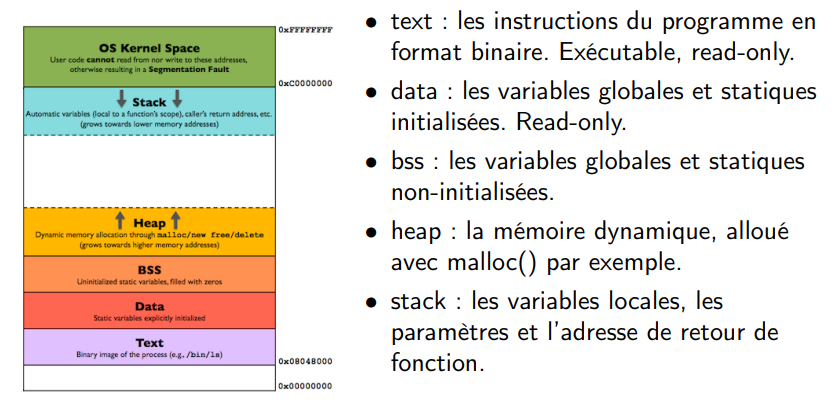
\includegraphics[width=17cm]{images/image_2021-12-30_131740.png}  
\end{center}
Assembleur = Langage intermédiaire entre le binaire et le code source
\newpage
\subsection{Vulnérabilités}
\subsubsection{Dénifitions}
\begin{itemize}[label = \textbullet, font = \Large]
    \item Deadlock :\\
    Lorsque chacun des programmes n'est plus en mesure d'effectuer une action attendant tous une ressource. (Cause : obtention simultanée et accès exclusif)\\\\
    \item Race condition :\\
    Lorsque 2 thread/processus accèdent à une ressource en même temps, étant donné qu'ils auront tous les 2 lu les données avant l'écriture, celle-ci vont procéder au même calcul et donc donner un résultat erroné. Exemple : A et B lisent un entier, tous 2 retiennent 17 et l'incremente de 1. La valeur écrite sera donc 18 au lieu de 19 si les 2 threads avaient s'étaient suivi.\\ Solutions : Utiliser des locks (accès exclusif). \\\\
    \item Fork bomb :\\
    Boucle de fork amenant au remplissage de la table des processus ainsi que toute la mémoire disponible.\\\\
    \item Memory Leak :\\
    Pas de libération de la mémoire louée dynamiquement dans la heap (par un malloc par exemple).\\\\
    \item Dangling pointers :\\
    Mémoire de pointeur libéré mais toujours disponible. Peut aussi être due en utilisant l'adresse d'une variable n'existant que dans une fonction.\\\\
    \item Segmentation fault :\\
    Déréférencement de NULL ou buffer overflow. (Lecture/Ecriture dans de la mémoire protégée)\\\\
    \item Stack buffer overflow :\\
    Ecrit plus de donnée que possible. Si il s'agit d'une variable locale = stack. Trop de donnée = débordement sur la frame actuelle, peut-être sur la frame précédente, l'adresse de retour et encore la frame précedente. Si l'on veut comparer la figure suivante avec le schéma de la mémoire présenté dans les premières pages, il nous faut alors mettre celle-ci à l'envers pour être dans le même sens.
        \begin{center}
            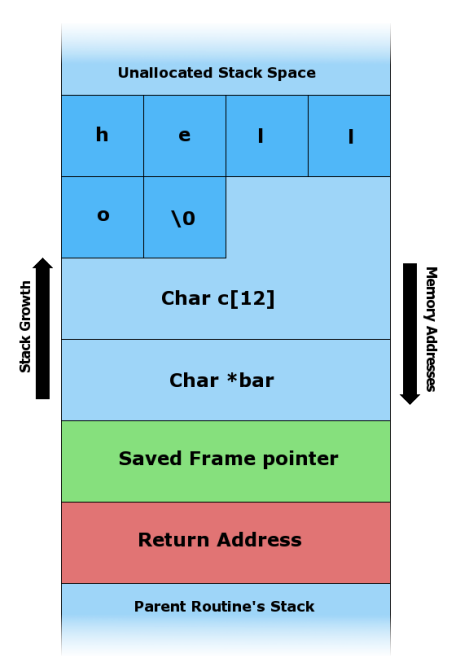
\includegraphics[width=4.8cm]{images/image_2021-12-30_141422.png}
        \end{center}
    \item  Time/Event bomb :\\
    Action malveillante se déclenchant à un évènement ou après un certain temps.\\\\
    \item Code injection :\\
    Le code exécute l'entrée utilisateur.\\\\
    \item Zip bomb :\\
    2 types :
    \begin{itemize}
        \item recursif (peut-être bloqué par un unpacker ou même un anti-virus)
        \item non-recursif (beaucoup plus subtil)
    \end{itemize}
    Va saturer le système lors de la décompression (mémoire, puissance de calcul).\\\\
    \item XML bomb :\\
    Chaque entité du XML peut faire référence à toutes les autres entités et ce un certain nombre de fois. (Example : Entité 9 appelle les 8 autres et la 8ème appelle les 7 autres et etc...)\\\\
    \item YAML bomb : 
    Pareil que la XML bomb.\\\\
    
\end{itemize}

\subsubsection{Race condition : Time of check/Time of use}
\begin{enumerate}
    \item Le fichier à modifier possède des droits SUID
    \item Temps de pause entre lecture des droits (time of check) et écriture dans le fichier (time of use). Peut-être causé par l'attente d'une entrée utilisateur ou un simple sleep().
    \item Possibilité de remplacer, durant ce délai, le fichier par un symlink vers un fichier que l'on veut modifier
\end{enumerate}

\subsubsection{Stack smashing}
Peut survenir si :
\begin{enumerate}
    \item Exploitation d'un stack buffer overflow
    \item L'attaquant connaît la taille du buffer à remplir
    \item Il peut construire les données à copier de façon à remplacer l'adresse de retour par une adresse de son choix
\end{enumerate}
Il peut alors simplement insérer du code exécutable, et modifier l'adresse de retour par l'adresse vers le code injecté. Il peut ainsi injecter du code ayant les mêmes droits que ceux du programme.
\begin{center}
    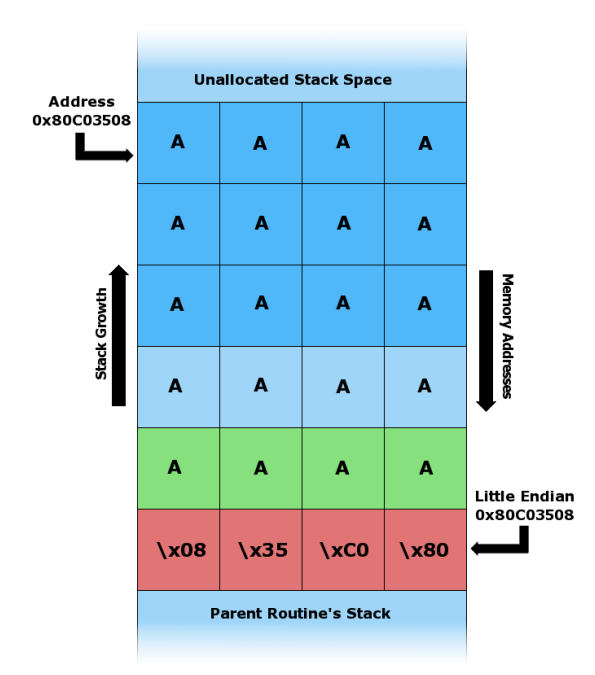
\includegraphics[width=6cm]{images/image_2021-12-30_142146.png}
\end{center}
Solutions :
\begin{itemize}[label = \textbullet, font = \Large]
    \item Stack non exécutable (-z execstack)
    \item Canaris : flag avant l'adresse de retour (-fno-stack-protector)
    \item ASLR : emplacement random dans la mémoire à chaque execution (echo '0' > /proc/sys/kernel/randomize\_va\_space)
\end{itemize}
Peuvent être contournées mais difficilement.

\subsubsection{Format string vulnerability}
Danger : utilisation de printf() en mettant directement la variable sans utiliser de formatage.\\\\ Possibilité donc de :
\begin{itemize}[label = $\hookrightarrow$, font = \Large]
    \item Afficher la stack :\\
    \begin{example}
    \$ ./a.out \$(python -c 'print "\%08x" * 32')
    \end{example}
    Format\%x affiche la valeur en hexa. Si rien n'est fourni à printf comme valeur, la fonction va récupérer les valeurs de la stack.
    \item Crash :\\
    \begin{example}
    \$ ./a.out \$(python -c 'print "\%s" * 100')
    \end{example}
    Format \%s est utilisé pour afficher une chaine de caractère, à partir d’un
    pointeur. Sans valeurs, printf va utiliser les valeurs de la stack
    comme pointeurs, ce qui mêne rapidement à une segfault.
    \item Accès à la mémoire arbitraire :\\
    \begin{example}
    \$ ./a.out \$(python -c 'print <address> + "\%x" * n + "\%s"')
    \end{example}
    Comme notre argument de programme se retrouve sur la stack, nous
    pouvons y écrire une adresse. Et comme nous disposons de \%s, qui
    affiche le contenu présent à une adresse, il est possible d’afficher la
    mémoire de toute adresse donnée. Il s’agit simplement de trouver le
    bon nombre de bytes à retirer de la stack avant notre adresse.
    \item Écriture dans la mémoire :\\
    \begin{example}
    \$ ./a.out \$(python -c 'print <address> + "\%x" * n + "\%n"')
    \end{example}
    L’idée est identique à l’accès à la mémoire mais le \%n va écrire le
    nombre de caractères affichés précédemment (entier) à l’adresse du
    paramètre fourni, autrement dit l’adresse que nous avons écrite sur
    la stack.
\end{itemize}

\newpage
\section{Analyse}
\subsection{Statique}
\subsubsection{Basique}
Analyse dans accéder au code source :
\begin{itemize}[label = \textbullet, font = \Large]
    \item strings (Extraction des strings)
    \item file (Analyse du fichier binaire)
    \item Vérifier les permissions
    \item Metadata (exiftool)
    \item Antivirus (virustotal, ClamAV, etc.) :\\
    Conseillé d'en utiliser plusieurs, ce que fait virustotal. Il existe 2 stratégies :
    \begin{enumerate}
        \item Statistique : Hash comparé à une base virale.
        \item Heuristique : Vérifier le comportement du programme pour trouver des opérations suspectes (possibilité de faux-positif).
    \end{enumerate}
\end{itemize}
\subsubsection{Avancée}
Analyse sans exécution du code source :
\begin{itemize}[label = \textbullet, font = \Large]
    \item Ouverture du code source (si possible)
    \item Ghidra (Décompilateur : fournit le code source)
    \item GDB (Désassembleur : fournit le langage d'assemblage)
    \item IDA (Désassembleur : fournit le langage d'assemblage)
    \item Decompile++ (Pour Python bytecode)
    \item Analyseur de code (Pylint, RATS, etc.)
    \item A la main :
    \begin{itemize}[label = $\hookrightarrow$, font = \Large]
        \item Les librairies et fonctions utilisées
        \begin{itemize}
            \item eval, exec, etc...
            \item strcpy (écriture en mémoire)
            \item printf, scanf
            \item sys, os, etc.
        \end{itemize}
        \item Les entrées/sorties
        \begin{itemize}
            \item provenance (utilisateur, fichier, socket)
            \item validation
            \item droits de lecture ou écriture
            \item destination
            \item infos sensibles en clair
        \end{itemize}
        \item Interactions avec le système
        \begin{itemize}
            \item commandes ou executables externes
            \item réseaux (socket, ftp, etc.)
            \item périphériques
            \item lecture, ecriture, copie, etc.
            \item variables d'environnement
        \end{itemize}
    \end{itemize}
\end{itemize}
\subsection{Dynamique}
\subsubsection{Basique}
Analyse durant l'exécution du programme, dans un environnement contrôlé (sandbox) :
\begin{itemize}[label = \textbullet, font = \Large]
    \item top
    \item ps aux
    \item pmap
    \item pidstat
    \item /proc/<PID>/status
    \item /proc/<PID>/FD (permet de voir des fichiers en cours de lecture/modification/création)3
    \item lsof (affiche tous les fichiers utilisés sur le système par tous les process)
    \item printenv (regshot sur Win) permet d'afficher les variables d'environnement. Il peut être intéressant de faire hash avant et après pour voir si il y a eu un changement
    \item strace
    \item autres outils d'analyse des processus
    \item Fuzzing (ex: boofuzz, radamsa)
    \item Réseaux : Wireshark, netstat, ss, fuser
\end{itemize}
\subsubsection{Avancée}
Analyse durant l'exécution du programme, grâce à un debugger pour inspecter la mémoire  (ex: GDB).

\subsection{Contre-mesure à l'analyse}
\begin{itemize}[label = \textbullet, font = \Large]
    \item Anti-disassembly\\
    Introduction de code difficile à comprendre (ex: double jump conditionnel) voire incorrect.
    \item Anti-debug :\\
    Modifier le comportement d'un programme si il passe dans un debugger. L'execution dans un debugger est différente et même parfois détectable grâce à des API de l'OS (windows).
    \item Anti-VM : \\
    L'execution dans une VM est facilement détectable et peu donc modifier son comportement pour paraître innofensif.
    \item Obfuscation : \\
    Rendre le code insupportable à lire pour brouiller les pistes (ex : brainfuck)
    \item Unpacking : \\
    Programme se présentant sous forme d'un package executable. Évite l'analyse du code exécutable malveillant.
\end{itemize}




\newpage
\section{Prévention}
La conception d'un programme doit être basé sur la sécurité.
Importance de la \emph{Security by design} :
\begin{itemize}[label = \textbullet, font = \Large]
    \item Hardening : \\
    Limiter les surfaces d'attaque : HTTP to HTTPS, limiter les entrées (barre de recherches par ex), diviser les services plutôt qu'une seule grosse application.
    \item Least Privilege : \\
    Pas de shell root, pas de connexion avec un compte admin sur les services mais un compte juste suffisant (ex : db), pas d'accès en lecture sur tout le FS
    \item Security by default :\\
    Si le niveau de sécurité peut être modifié, le niveau de sécurité doit être le plus élevé par défaut. (utilisation de rôle au lieud d'un compte admin, https, port aléatoire, etc.)
    \item Defense in depth :\\
    Ne pas se contenter d'une seule vérification de sécurité. Ex : Même si il s'agit d'un intranet, il faut tout de même s'identifier pour accéder au réseau. (2FA, Vérification systématique des droits, etc.)
    \item Failing securely :\\
    Si jamais une erreur doit survenir pendant le dérouleement d'une vérification de droits, la fonction doit refuser les droits par défaut et ne pas laisser le rôle "à déterminer" (ex : try return isAdmin(); except return False;).
    \item Avoid external trust :\\
    Méfiance envers les services externes à notre contrôle (API, ISP, CDN, etc.)
    \item Seperation of duty : \\
    Utilisation typique : 
        \begin{itemize}[label = $\hookrightarrow$, font = \Large]
            \item Une entité contrôle si l'action peut être effectuée (ex: droit, ACL, etc.)
            \item Une entité fait l'action (ex: user)
            \item Une entité note l'action effectuée (ex: logging)
        \end{itemize}
    De cette manière on évite qu'une entité fasse quelque chose et le cache de lui même.
    \item KISS = \textbf{K}eep \textbf{I}t \textbf{S}imple \textbf{S}tupid :\\
    Le système doit être le plus simple possible. Plus il est complexe, plus il sera difficile de le comprendre et ne le sécuriser.
    \item Avoid security by obscurity\\
    Ne jamais croire que rendre la lecture d'un programme difficile le rend sécurisé. But ? Décourager !
    \item Open Security (Principe de Kerchoff)
    Dans tout programme, partir du principe que l'attaquant en aura la même connaissance que nous. Seul la clé doit rester secrète. Ce principe dirige naturellement vers la mise à disposition de tous du code source (open-source). Cela peut avoir un impact important sur la sécurité :
    \begin{itemize}[label = $\hookrightarrow$, font = \Large]
        \item S'assurer qu'il a bien été conçu et que la divulgation ne constitue pas un risque
        \item Les failles de sécurité s'y trouvant ont plus de chances d'être découvertes et corrigées
    \end{itemize}
    \item Safe language : 
    \begin{itemize}
        \item Adapté
        \item Memory safe (pas du C kappa)
        \item Typage sûr (en général, un typage fort et statique est considéré comme plus sûr. Par exemple le JavaScript est tout sauf un language au typage sûr)
    \end{itemize}
    \item Defensive programming :\\
    Tout ce qui peut mal se passer doit être pris en compte :\begin{itemize}
        \item Inputs (valider le format et faire de la sanitization)
        \item Erreur (Gérer les erreurs grâce à des exceptions)
        \item Cas exceptionnels (Liste vide, division par 0, tri avec doublons, etc.)
        \item Passer par des batteries de tests. Son importance à amené au TDD (Test driven development) : Avant d'écrire du code, les tests sont créé pour vérifier les spécifications de la méthode ou fonction.
        \item etc.
    \end{itemize}
\end{itemize}
\newpage



\section{Défense}
\subsection{Stratégie de protection}
Règle numéro 1 : Tout logiciel doit être traité comme une menace potentielle ! C'est pour cela que tout logiciel doit avoir accès aux ressources juste nécessaire, pas plus pas moins.\\\\
Bonnes pratiques et stratégies de protection :
\begin{itemize}[label = \textbullet, font = \Large]
    \item Pour chaque logiciel, créer un utilisateur et un groupe.
    \item Limiter l'accès de cet utilisateur au FS.
    \item Si le logiciel est lancé par un autre utilisateur, passer sur son utilisateur attribué dès que possible (setuid() \& setgid()).
    \item Si besoin de droits admin, s'assurer que les droits soient relâché dès que possible !
    \item Limiter les ressources matérielles (/etc/security/limits.conf, ulimit \& quotatool). Le but est d'empêcher le DOS.
    \item Bonne gestion du réseaux en mettant par exemple :
    \begin{itemize}
        \item la création d'alerte lors d'une communication suspecte
        \item les iptables pour restreindre certain utilisateurs/processus (module \emph{owner})
        \item le monitoring des requêtes DNS
    \end{itemize}
    \item Le sandboxing :
    \begin{itemize}
        \item Jailing avec Chroot :\\
        Fournir une version restreinte du système en modifiant la racine du système de fichiers. Possibilité de modifier également le PATH enlever des exécutables. Idéal pour un hébergement mutualisé/virtualisé (plusieurs sites sur le même serveur).
        \item Machine virtuelle :\\
        Simulation d'un système complet. Une faille dans l'hyperviseur pourrait permettre à un malware de sortir. De plus, celui-ci peut adopter un comportement différent quand il est dans une VM.
        \item Containers :\\
        Entre le jailing et la VM. Basés sur les cgroups qui attribuent des restrictions à un groupe de processus, ils permettent l’exécution de processus complètement isolés des autres mais utilisant les capacités du même système hôte.
    \end{itemize}
    \item Sauvegarde de données : \\
    \begin{itemize}
        \item Facile à metre en place et à restaurer
        \item Double copie (locale et distante)
        \item Fréquence suffisante
        \item Conservation dans le temps suffisante
    \end{itemize}
    \item Sauvegarde du système : \\
    \begin{itemize}
        \item Système bare metal : image des partitions systèmes
        \item Système virtuel : snapshots ou copie des disques
    \end{itemize}
    \item Mettre en place des solutions de remote logging
\end{itemize}

\subsection{Contre quoi se défendre ?}
\begin{itemize}[label = \textbullet, font = \Large]
    \item Tout applicatif ou logiciel qui permet une violation du CIA (Confidentiality/Integrity/Availability). 
    \item Tous les logiciels posent des menaces plus ou moins importantes
\end{itemize}

\subsection{Menaces}
\begin{itemize}[label = \textbullet, font = \Large]
    \item Lecture de données
    \item Modification des données
    \item Espionnage de l'activité
    \item Détournement de ressources matérielles (ex : minage)
    \item Déni de service
    \item Spoofing
    \item etc.
\end{itemize}

\subsection{Définition d'un logiciel menaçant}
Une telle définition n'existe pas car cela dépend du contexte et du cas d'utilisation.

\subsection{Detection par logiciel}
La détection de logiciel malveillant de manière parfaite est impossible à l'aide d'une machine

\newpage
\section{Pratique}
\subsection{GDB}
Commandes utiles :
\begin{itemize}[label = \textbullet, font = \Large]
    \item disassemble <function>
    \item run
    \item break <fonction/ligne> : ajout de breakpoint
    \item continue : continue après le break
    \item print \&<x> : affiche m'adresse d'une variable/fonction
    \item print *<x> : affiche la valeur d'une variable/fonction
    \item x/<n> \&<y> : affiche n bytes après l'adresse de y
    \item x/<n><o> \$rsp : afficher n bytes de la stack sous forme de o :
    \begin{itemize}
        \item d : signé
        \item x : hexa
        \item u : non-signé
    \end{itemize}
\end{itemize}

\subsection{Comment faire un stack smashing}
Partons du principe qu'on le sait déjà vulnérable :
\begin{enumerate}
    \item Calculer le buffer :
    \begin{itemize}
        \item GDB
        \begin{itemize}
            \item Ouvrir le binaire avec gdb
            \item Mettre un break après le strcpy et run du padding en argument
            \item print \$rsp
            \item print \$rbp
            \item Grâce à \emph{x/100xg \$rsp}, repérer notre buffer et compter le nombre de byte restant jusqu'à arriver à l'adresse de \$rbp.
            \item Noter également l'adresse du debut de notre buffer
            \item La taille du buffer = nombre de caractère mis en argument + le nombre compté
        \end{itemize}
        \item La taille du buffer peut être plus facilement trouvée grâce a Ghidra
    \end{itemize}
    \item Taille du padding = Taille du buffer + taille RBP (8) - taille du code
    \item Commande finale :\\
    \begin{example}
    ./binary \$(python -c '<code> + "A" * <Taille padding> + <adresse du buffer>[::-1]')
    \end{example}
    L'adresse du buffer doit s'écrire de manière à ce que 0x7ffffffdee0 devienne : "\textbackslash x7f\textbackslash xff\textbackslash xff\textbackslash xff\textbackslash xde\textbackslash xe0". Le little-endian se fait grâce à [::-1]
\end{enumerate}
Il est important de savoir qu'à cause des variables d'environnements différentes entre gdb et votre shell, l'adresse du buffer n'est pas la même. Voilà pourquoi toute cette explication ne sert à rien.

\subsection{Exemple de tests en python}
\begin{center}
    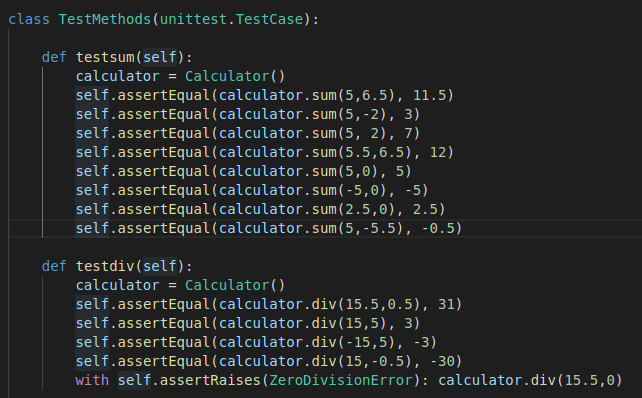
\includegraphics[width=0.89\textwidth]{images/image_2021-12-31_193315.png}
\end{center}
Lancement des tests avec : unittest.main()

\subsection{Comment faire du jailing}
\begin{enumerate}
    \item Créer le dossier du chroot et mettre root comme owner :\\
    \begin{example}
    \# mkdir /home/jail\\[0.1cm]
    \# chown root:root /home/jail
    \end{example}
    \item Lister et copier tous les fichiers nécessaires au lancement d'un shell et des commandes voulues dans le dossier précédemment créé :\\
    \begin{example}
    \# ldd /bin/\{bash, ls, cp, rm\}\\[0.1cm]
    \# mkdir /home/jail/\{bin,lib64,lib\}\\[0.1cm]
    \# cp /bin/bash /home/jail/bin\\[0.1cm]
    \# cp /lib/lib/x86\_64-linux-gnu/libtinfo.so.5 /home/jail/lib/\\[0.1cm]
    etc.
    \end{example}
    \item Créer le/les utilisateur(s) et/ou le groupe
    \begin{example}
    \# groupadd jail (facultatif)\\[0.1cm]
    \# useradd myuser\\[0.1cm]
    \# passwd myuser\\[0.1cm]
    \# usermod -aG jail myuser (facultatif)
    \end{example}
    \item Ajouter les lignes suivantes à la fin du fichier /etc/ssh/sshd\_config (mettre User ou group dépendant de votre cas):\\
    \begin{example}
    Match User(/group) myuser(/jail)\\
    ..........ChrootDirectory /home/jail
    \end{example}
    \item Vérifier que le shell par défaut de/des utilisateur(s) soit bien celui ajouté au dossier /home/jail
\end{enumerate}

\subsection{Retrouver les arguments dans la mémoire - GDB}
\begin{enumerate}
    \item \emph{break main}
    \item \emph{info frame} :
    \begin{center}
        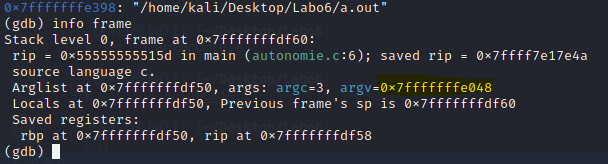
\includegraphics[width=0.80\textwidth]{images/image_2022-01-01_160339.png}
    \end{center}
    \item On lit les données à ces emplacements mémoire. J'ai personnellement eu des adresses à cette endroit dans la mémoire :
    \begin{center}
        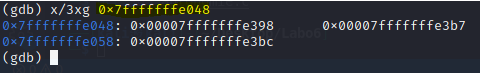
\includegraphics[width=0.80\textwidth]{images/image_2022-01-01_160559.png}
    \end{center}
    \item Il ne suffit plus que de lire le contenu de ces adresses :
    \begin{center}
        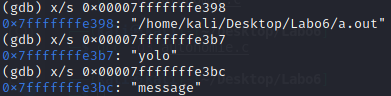
\includegraphics[width=0.80\textwidth]{images/image_2022-01-01_160726.png}
    \end{center}
\end{enumerate}

\subsection{Attaque par format string}
\begin{enumerate}
    \item Code vulnérable :
    \begin{center}
        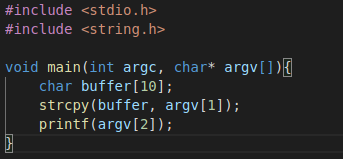
\includegraphics[width=0.30\textwidth]{images/image_2022-01-01_161712.png}
    \end{center}
    \item Afficher la stack et lire l'hexadecimal :
    \begin{example}
    \$ ./a.out "petit-test" "`python -c "print '\%lx' * 10 "`" 
    \end{example}
\end{enumerate}
\begin{center}
        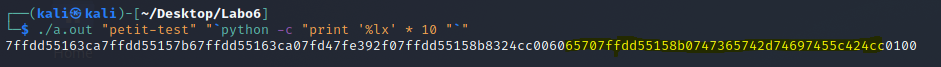
\includegraphics[width=0.99\textwidth]{images/image_2022-01-01_163338.png}
        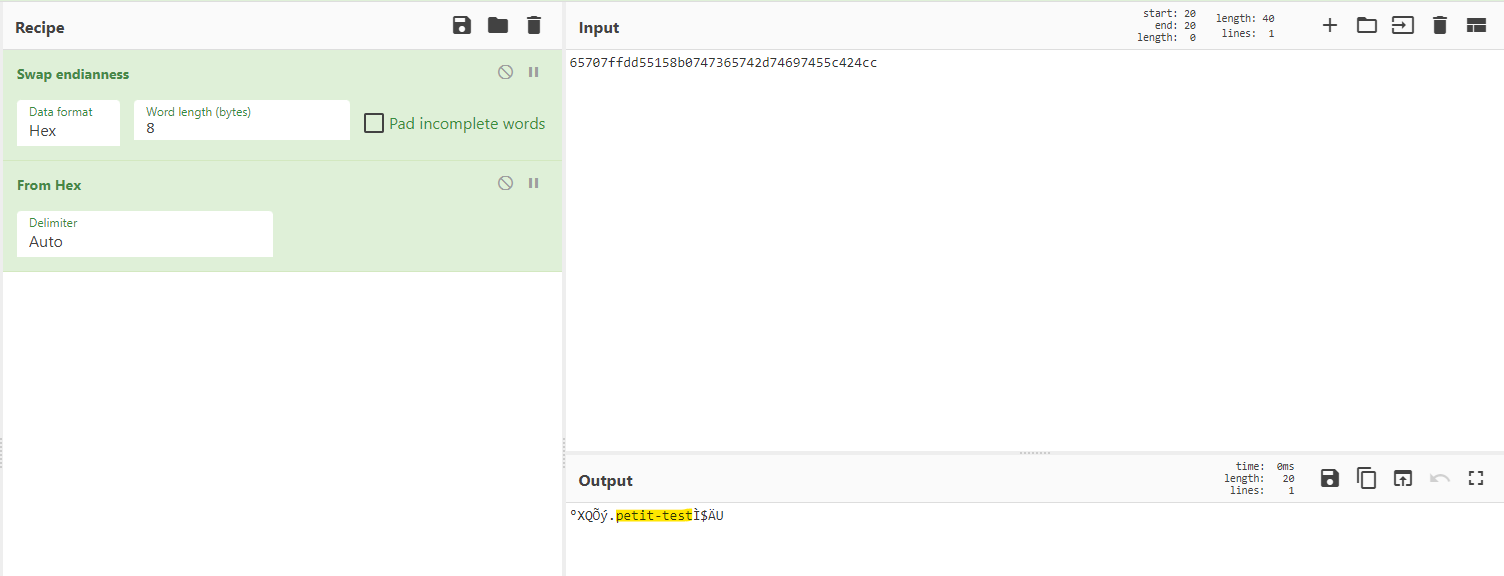
\includegraphics[width=0.99\textwidth]{images/image_2022-01-01_163502.png}
\end{center}

\subsection{Créer un daemon DNS Monitoring}
\begin{enumerate}
    \item Créer un groupe ayant les droits de lancer tcpdump ainsi qu'un utilisateur dans ce groupe :
    \begin{example}
    \# groupadd pcap\\[0.1cm]
    \# usermod -aG pcap <user> \\[0.1cm]
    \# chgrp pcap /usr/bin/tcpdump\\[0.1cm]
    \# setcap cap\_net\_raw,cap\_net\_admin=eip /usr/bin/tcpdump\\[0.1cm]
    \# ln -s /usr/bin/tcpdump /usr/local/bin/tcpdump
    \end{example}
    \item Créer un service dans \emph{/lib/systemd/system/<nom>.service} et y mettre une configuration comme celle-ceci :
    \begin{example}
    $[$Unit$]$\\After=network.target\\\\$[$Service$]$\\ExecStart=/usr/bin/tcpdump -i eth0 ip and 'port 53' -w /home/mypcap/output.pcap\\Type=simple\\\\$[$Install$]$\\WantedBy=multi-user.target
    \end{example}
\end{enumerate}

\subsection{Auditd}
\begin{enumerate}
    \item Ajouter auditd au grub
    \begin{enumerate}
        \item Ouvrir /etc/default/grub
        \item Modifier la ligne GRUB\_CMDLINE\_LINUX\_DEFAULT en y ajoutant "audit=1"
        \item Update le grub avec :\\
        \begin{example}
        \# grub-mkconfig -o /boot/grub/grub.cfg
        \end{example}
    \end{enumerate}
    \item systemctl enable auditd
    \item Exemple de règles temporaires :
    \begin{itemize}
        \item auditctl -w /etc/passwd -p rwa
        \item auditctl -a always,exit -S all -F uid=1002
        \item auditctl -a always,exit -F arch=b64 -S chmod,open,kill -k test\\ (-k sert à lier le log avec une clé afin de le retrouver plus facilement)
    \end{itemize}
    \item Pour créer des règles permanentes, il suffit d'ajouter les options dans le fichier /etc/audit/rules.d/audit.rules et de redémarrer le service.
    \item Lire le résultat de l'audit dans /var/log/audit/audit.log
\end{enumerate}

\subsection{Limiter l'espace disque d'un utilisateur avec un disque virtuel}
\begin{enumerate}
    \item Créer un dossier dans /media/ :
    \begin{example}
    mkdir /media/test
    \end{example}
    \item Copier et convertir /dev/zero en une image avec les quotas requis :
    \begin{example}
    dd if=/dev/zero of=/media/test/client.img bs=512k count=200
    \end{example}
    \item Formater ce disque :
    \begin{example}
    mkfs.ext4 /media/test/client.img
    \end{example}
    \item Créer le répertoire et monter le disque :\
    \begin{example}
    mkdir /home/quotatest\\ mount -o loop /media/test/client.img /home/quotatest
    \end{example}
    \item Pour rendre ce montage permanent, modifier /etc/fstab en rajoutant ce qui suit :
    \begin{example}
    /media/test/client.img /home/client ext4 loop 0 2
    \end{example}
    \item Créer l'utilisateur et le nommer propriétaire de son home:
    \begin{example}
    adduser quotatest\\
    chown -R quotatest:quotatest /home/quotatest
    \end{example}
\end{enumerate}























\end{document}